\documentclass{article}
\usepackage[utf8]{inputenc}
\usepackage{hyperref}
\usepackage{subfig}
\title{FYS4150 Project 1}
\author{Jens Bratten Due }
\date{September 2019}

\usepackage{natbib}
\usepackage{graphicx}
\usepackage{amsmath}
\begin{document}

\maketitle
\section{Abstract}
This project investigates the efficiency and precision of three different algorithms for solving the one-dimensional Poisson equation. The first two algorithms are general and specialized cases of solving a tri-diagonal matrix, and the last is the LU-decomposition. After running the algorithms on differently sized matrices, it was found that all algorithms satisfactorily solved the problem for smaller dimensions $n < 10^5$. However, the LU-decomposition failed at higher n, leading to exceeded memory usage, crashing the program. The first two algorithms had no problems with this and proved sufficient for up to at least $n = 10^7$ grid points. The specialized algorithm was estimated to need half the amount of FLOPS (floating point operations) compared to the general algorithm. This was confirmed by timing the algorithms in our C++ programs (found at GitHub address \url{https://github.com/jensbd/FYS4150/tree/master/Project1}). Relative error for the specialized algorithm was also calculated, showing, as expected, the smallest errors for higher n, up until $n = 10^7$ where the error term blew up due to round-off errors caused by limited machine precision.

\section{Introduction}
The aim of this project is too study the use of different algorithms for solving a set of linear equations. This specific set arises from discretizing the one-dimensional Poisson equation with Dirichlet boundary conditions.
\begin{equation}
    -u''(x) = f(x), \hspace{0.5cm} x\in(0,1), \hspace{0.5cm} u(0) = u(1) = 0
\end{equation}
Three algorithms will be presented, one general algorithm, one specialized and lastly the LU-decomposition.
Firstly, the derivation of the algorithms is presented before the results are shown and discussed. 

\section{Method}
\textbf{1a)}\\
The discretized equation is
\begin{equation}
    -\frac{v_{i+1}+v_{i-1}-2v_i}{h^2} = f_i  \hspace{0.5cm} \mathrm{for} \hspace{0.1cm} i=1,\dots, n,
\end{equation}
The set of linear equations arises by writing this out for each i.
\begin{equation}
    \begin{gathered}
    -v_2 + 2v_1 = h^2f_1 \\
    -v_3 - v_1 + 2v_2 = h^2f_2 \\
            \vdots\\
    -v_n - v_{n-2} + 2v_{n-1} = h^2f_{n-1}\\
     - v_{n-1} + 2v_{n} = h^2f_{n}
    \end{gathered}
\end{equation}
With the boundary conditions $v_0 = v_{n+1} = 0$. These can then be written as a tridiagonal matrix:
\begin{equation}
    \begin{bmatrix}
                           2& -1& 0 &\dots   & \dots &0 \\
                           -1 & 2 & -1 &0 &\dots &\dots \\
                           0&-1 &2 & -1 & 0 & \dots \\
                           & \dots   & \dots &\dots   &\dots & \dots \\
                           0&\dots   &  &-1 &2& -1 \\
                           0&\dots    &  & 0  &-1 & 2 \\
                      \end{bmatrix}
            \begin{bmatrix}
        v_1\\v_2\\v_3\\\vdots\\v_n
    \end{bmatrix}
    = h^2\begin{bmatrix}
        f_1\\f_2\\f_3\\\vdots\\f_n
    \end{bmatrix}
\end{equation}
\textbf{1b)}\\
We will now look at the general case where we do not know the matrix elements along the diagonals, and try to find the solutions to the linear equations by doing matrix operations. 
\begin{equation}
    \begin{bmatrix}
                           b_1& c_1 & 0 &\dots   & \dots &\dots \\
                           a_1 & b_2 & c_2 &\dots &\dots &\dots \\
                           & a_2 & b_3 & c_3 & \dots & \dots \\
                           & \dots   & \dots &\dots   &\dots & \dots \\
                           &   &  &a_{n-2}  &b_{n-1}& c_{n-1} \\
                           &    &  &   &a_{n-1} & b_n \\
                      \end{bmatrix}\begin{bmatrix}
                           v_1\\
                           v_2\\
                           \dots \\
                          \dots  \\
                          \dots \\
                           v_n\\
                      \end{bmatrix}
  =h^2\begin{bmatrix}
                           f_1\\
                           f_2\\
                           \dots \\
                           \dots \\
                          \dots \\
                           f_n\\
                      \end{bmatrix}
           \end{equation}
For easier visualization, we will show the operations as if $n = 4$. The first step is a forward substitution.
\begin{equation}
    \begin{bmatrix}
        b_1 & c_1 & 0 & 0 \\
        a_1 & b_2 & c_2 & 0 \\
        0 & a_2 & b_3 & c_3 \\
        0 & 0 & a_3 & b_4
    \end{bmatrix}
    \begin{bmatrix}
        v_1 \\ v_2 \\ v_3 \\v_4
    \end{bmatrix}
    =h^2\begin{bmatrix}
        f_1\\
        f_2\\
        f_3\\
        f_4
    \end{bmatrix}
\end{equation}
To remove $a_1$, we multiply the first row with $a_1/b_1$ and subtract from the second row: 
\begin{equation}
    \begin{bmatrix}
        b_1 & c_1 & 0 & 0 \\
        0 & b_2 - \frac{c_1a_1}{b_1} & c_2 & 0 \\
        0 & a_2 & b_3 & c_3 \\
        0 & 0 & a_3 & b_4
    \end{bmatrix}
    \begin{bmatrix}
        v_1 \\ v_2 \\ v_3 \\v_4
    \end{bmatrix}
    =h^2\begin{bmatrix}
        f_1\\
        f_2 - \frac{f_1a_1}{b_1}\\
        f_3\\
        f_4
    \end{bmatrix}
\end{equation}
We set $ b_2 - \frac{c_1a_1}{b_1}= b_2^*$, $f_2 - \frac{f_1a_1}{b_1} = f_2^*$ and continue until the a-diagonal is removed.
\begin{equation}
    \begin{bmatrix}
        b_1^* & c_1 & 0 & 0 \\
        0 & b_2^* & c_2 & 0 \\
        0 & 0 & b_3^* & c_3 \\
        0 & 0 & 0 & b_4^*
    \end{bmatrix}
    \begin{bmatrix}
        v_1 \\ v_2 \\ v_3 \\v_4
    \end{bmatrix}
    =h^2\begin{bmatrix}
        f_1^*\\
        f_2^*\\
        f_3^*\\
        f_4^*
    \end{bmatrix}
\end{equation}
After this step, we have the following variables.
\begin{equation}
    \begin{gathered}
    b_1^*= b_1  \\
    b_i^* = b_i - \frac{c_{i-1}a_{i-1}}{b_{i-1}^*}  \\
    f_1^* = f_1  \\
    f_i^* = f_i - \frac{f_{i-1}^*a_i}{b_i}
    \end{gathered}
\end{equation}
From here, we perform a backward substitution to remove the c-diagonal. We multiply the last row with $c_3/b_4^*$ and subtract from the third row.
\begin{equation}
    \begin{bmatrix}
        b_1^* & c_1 & 0 & 0 \\
        0 & b_2^* & c_2 & 0 \\
        0 & 0 & b_3^* & 0 \\
        0 & 0 & 0 & b_4^*
    \end{bmatrix}
    \begin{bmatrix}
        v_1 \\ v_2 \\ v_3 \\v_4
    \end{bmatrix}
    =h^2\begin{bmatrix}
        f_1^*\\
        f_2^*\\
        f_3^* - \frac{f_4^*c_3}{b_4^*}\\
        f_4^*
    \end{bmatrix}
    \rightarrow
\end{equation}
Defining $\Tilde{f}_3 = f_3^* - \frac{f_4^*c_3}{b_4^*}$ and continuing.
\begin{equation}
    \begin{bmatrix}
        b_1^* & c_1 & 0 & 0 \\
        0 & b_2^* & 0 & 0 \\
        0 & 0 & b_3^* & 0 \\
        0 & 0 & 0 & b_4^*
    \end{bmatrix}
    \begin{bmatrix}
        v_1 \\ v_2 \\ v_3 \\v_4
    \end{bmatrix}
    =h^2\begin{bmatrix}
        f_1^*\\
        f_2^* - \frac{\Tilde{f}_3c_2}{b_3^*}\\
        \Tilde{f}_3\\
        f_4^*
    \end{bmatrix}
    \rightarrow
\end{equation}
\begin{equation}
    \begin{bmatrix}
        1 & 0 & 0 & 0 \\
        0 & 1 & 0 & 0 \\
        0 & 0 & 1 & 0 \\
        0 & 0 & 0 & 1
    \end{bmatrix}
    \begin{bmatrix}
        v_1 \\ v_2 \\ v_3 \\v_4
    \end{bmatrix}
    =h^2\begin{bmatrix}
        \frac{\Tilde{f_1}}{b_1^*}\\
        \frac{\Tilde{f_2}}{b_2^*}\\
        \frac{\Tilde{f_3}}{b_3^*}\\
        \frac{\Tilde{f_4}}{b_4^*}
    \end{bmatrix}
\end{equation}
With $\Tilde{f_4} = f_4^*$. Finally, we have the completed linear equations.
\begin{equation}
    \begin{gathered}
        v_{i} = \frac{\Tilde{f_{i}}}{b_i^*} = \frac{f_{i}^* - v_{i+1}c_i}{b_i^*} 
    \end{gathered}
\end{equation}
And the endpoint $v_n = f_n^*/b_n^*$.
\newline The speed of this algorithm can be measured in the number of floating point operations (FLOPS) needed to compute the final solution. The forward substitution requires 1 pre-calculated factor $a_i/b_i$ per iteration, as well as 2 multiplications and 2 subtractions. This results in 5 FLOPS per iteration, for a total $5(n-1)$ FLOPS.
The backward substitution requires 1 pre-calculated factor $c_{i-1}/b_{i}^*$, 1 multiplication and 1 subtraction per iteration, resulting in $3(n-1)$ FLOPS.
Adding these gives us the final $8(n-1)$ FLOPS needed for the algorithm.
\newline
\newline
\textbf{1c)}\newline
Since we already know all a-, b-, and c-values, we can specialize our algorithm to improve efficiency. The a-, and c-values are unchanged through the algorithm, and the following modifications are possible. $a_i = -1, c_i = -1$, so
\begin{equation}
    \begin{gathered}
    b_1^* = 2\\
    b_i^* = 2 - \frac{1}{b_{i-1}^*} = \frac{i+1}{i}  \\
    f_1^* = f_1 \\
    f_i^* = f_i + \frac{(i-1)f_{i-1}^*}{i}
    \end{gathered}
\end{equation}
The final solution then becomes
\begin{equation}
    u_{i-1} = \frac{i-1}{i}(f_{i-1}^* + u_i)
\end{equation}
As for the efficiency of this specialized algorithm, both the forward and backward substitution now only requires 1 multiplication and 1 subtraction on the right hand side per iteration, resulting in a total of 4(n-1) FLOPS.\\\\
\textbf{1d)}\\
We will calculate the relative error like this:
\begin{equation}
    \epsilon_i=log_{10}\left(\left|\frac{v_i-u_i}
                 {u_i}\right|\right)
\end{equation}
and evaluate based on number of grid points n. We will use the specialized algorithm for this.\\\\
\textbf{1e)}\\
Lastly, we will compare our algorithms with the LU decomposition, a widely used algorithm for solving matrix problems. The LU decomposition uses a number of FLOPS proportional to $n^3$. [1]
\section{Results}
\subsection{Numerical and analytic differences}
In Figure 1, it is shown how the numerical approximation differs from the analytic solution as a function of the number of grid points n. At a high enough n, the numerical and analytic plots look very similar.

\begin{figure}[!h]
\centering
\subfloat[$n = 10$]{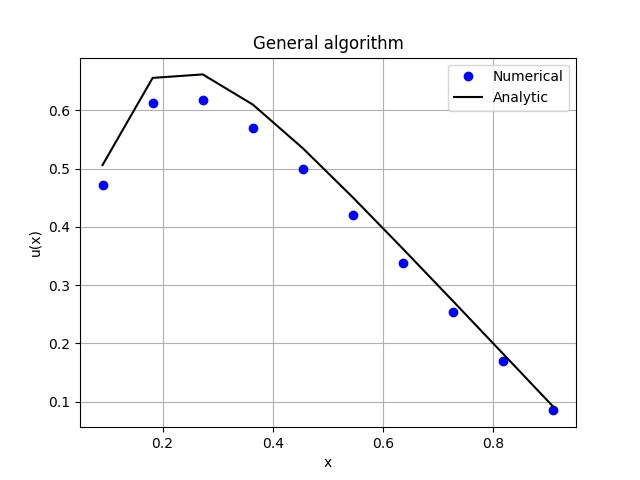
\includegraphics[scale=0.25]{10.jpg}}
\qquad
\subfloat[$n = 100$]{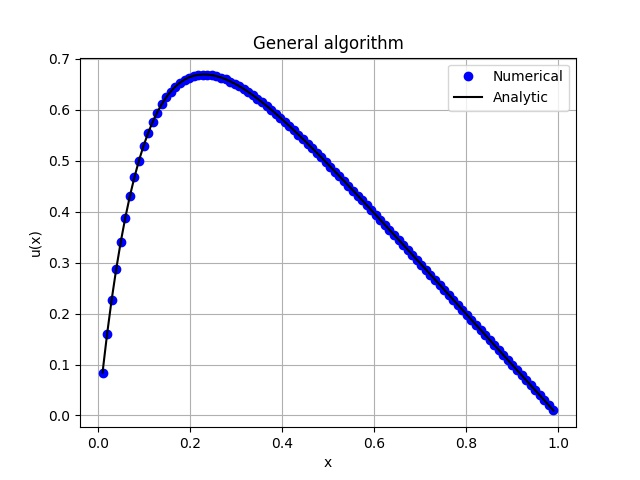
\includegraphics[scale=0.25]{100.jpg}}

\subfloat[$n = 1000$]{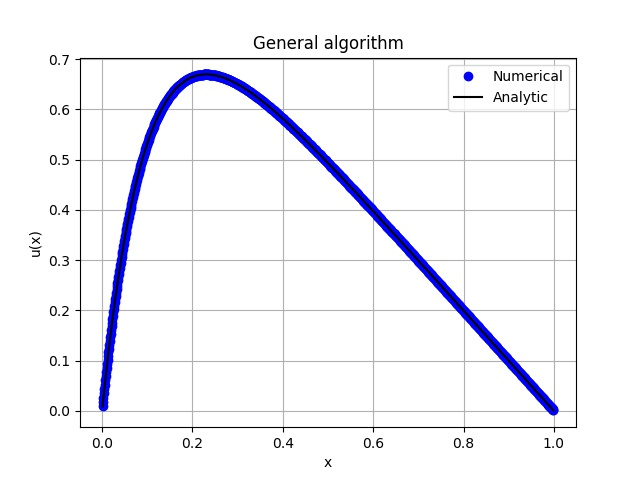
\includegraphics[scale=0.25]{1000.jpg}}

\caption{Figure showing the numerical and analytical solutions of our differential equation, with the number of grid points being n = 10, 100 and 1000. With increasing n, the numerical solution rapidly approaches the analytic.}
\label{fig:1)}
\end{figure}

\subsection{Relative error and CPU time}
In Table 1, one can see how the relative error and CPU time evolves with increasing number of grid points, and how they differ between our three algorithms.

\begin{table}[ht]
    \centering
    \begin{tabular}{c|c|c|c|c|c}
         \hline
         n & General time & Spec. time & LU time & Spec. error   \\
         \hline
         10 & - & - & -  &$10^{-1.10058}$ \\
         $10^2$ & - & - & 0.005s  &$10^{-3.0794}$ \\
         $10^3$ & - & - &0.01s  &$10^{-5.07918}$ \\
         $10^4$ & - & - & 0.77s &$10^{-7.07918}$ \\
         $10^5$ & 0.004s&0.0033s & Memory error &$10^{-9.08072}$  \\
         $10^6$ &0.034s &0.024s & Memory error &$10^{-11.504}$  \\
         $10^7$ & 0.322s & 0.184s & Memory error  & $INF$ \\
    \end{tabular}
    \caption{Table showing timings and errors for three tri-diagonal matrix solving algorithms. The times for small n were too short for our programs clock precision, registering only as 0 or 0.001. Note also that the error for $n = 10^7$ is infinite. This is due to machine precision not being good enough for these small numbers, generating round-off errors. The LU decomposition results in memory overflow at $n >= 10^5$. The LU decomposition of matrices of these dimensions requires $n^3 = 10^{15}$ FLOPS, making the machine quickly run out of available memory. }
    \label{tab:my_label}
\end{table}
\section{Conclusion}
Choice and optimization of algorithms can be detrimental for solving differential equations and linear algebra problems. We have seen how the LU decomposition very quickly can lead to memory overflows and high run times. Our algorithms has thusly proved to be a better choice for solving the one-dimensional Poisson equation. The specialized algorithm was estimated to require half the amount of FLOPS as the general, and the CPU times matched this estimation fairly well for larger matrices.
\section{Appendix}
All programs and results can be found here:
\url{https://github.com/jensbd/FYS4150/tree/master/Project1}

\section{Bibliography}
This report is made possible by lecture slides and code examples in the course, made available by Morten Hjorth-Jensen.\newline\newline
 [1] Hjorth-Jensen, M., n.d. Computational Physics Lectures: Linear Algebra methods 34. URL \\
 \url{http://compphysics.github.io/ComputationalPhysics/doc/pub/linalg/pdf/linalg-print.pdf}
\newline\newline 
 [2] Hjorth-Jensen, M., CompPhysics/ComputationalPhysicsMSU, 2019. URL\\ \url{https://github.com/CompPhysics/ComputationalPhysicsMSU}
\newline\newline 
 [3] Hjorth-Jensen, M., Overview of course material: Computational Physics. URL \url{http://compphysics.github.io/ComputationalPhysics/doc/web/course}

\end{document}
